\documentclass[12pt]{article}
\usepackage[margin=1.0in]{geometry}
\usepackage{setspace}
\usepackage{titling}

\usepackage{amsmath,amsthm,amssymb}
\usepackage{graphicx}
\usepackage{enumerate}
\usepackage[shortlabels]{enumitem}

\setstretch{1.5}
\setlength{\droptitle}{-8em}

\begin{document}

  \title{605.611 - Foundations of Computer Architecture \\ Assignment 03\vspace{-0.5em}}
  \author{Sabbir Ahmed}
  \maketitle
  \vspace{-1em}

  Do all the following in Logisim.  Problem 2 is extra credit.

  \begin{enumerate}
    \item Implement an 8-to-1 multiplexer using only 2-to-1 multiplexers.
    \begin{figure}[h]
      \centering
      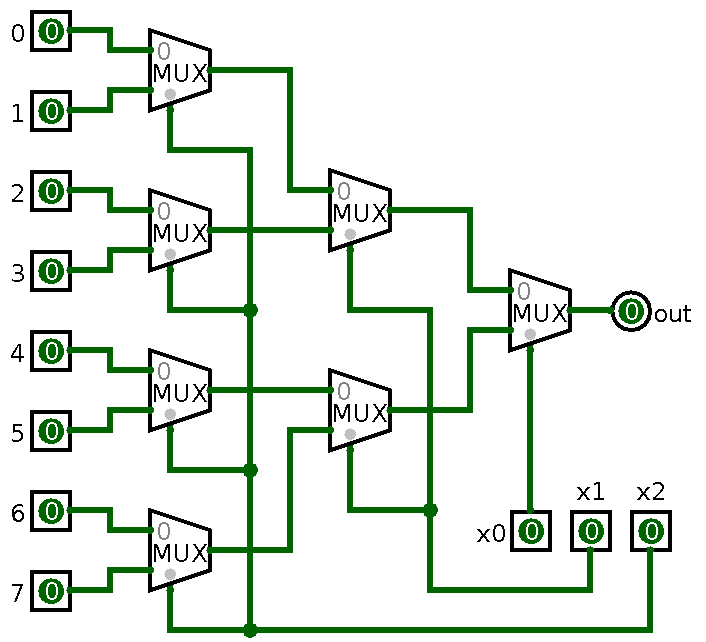
\includegraphics[width=0.5\textwidth]{assn/03/media/01.png}
      \caption{An 8-to-1 Multiplexer Using 2-to-1 Multiplexers in Logisim}
    \end{figure}
    \clearpage

    \item Implement a 16-to-4 encoder using only 8-to-3 encoders, a mux, and basic gates (AND, OR, and NOT).
    \begin{figure}[h]
      \centering
      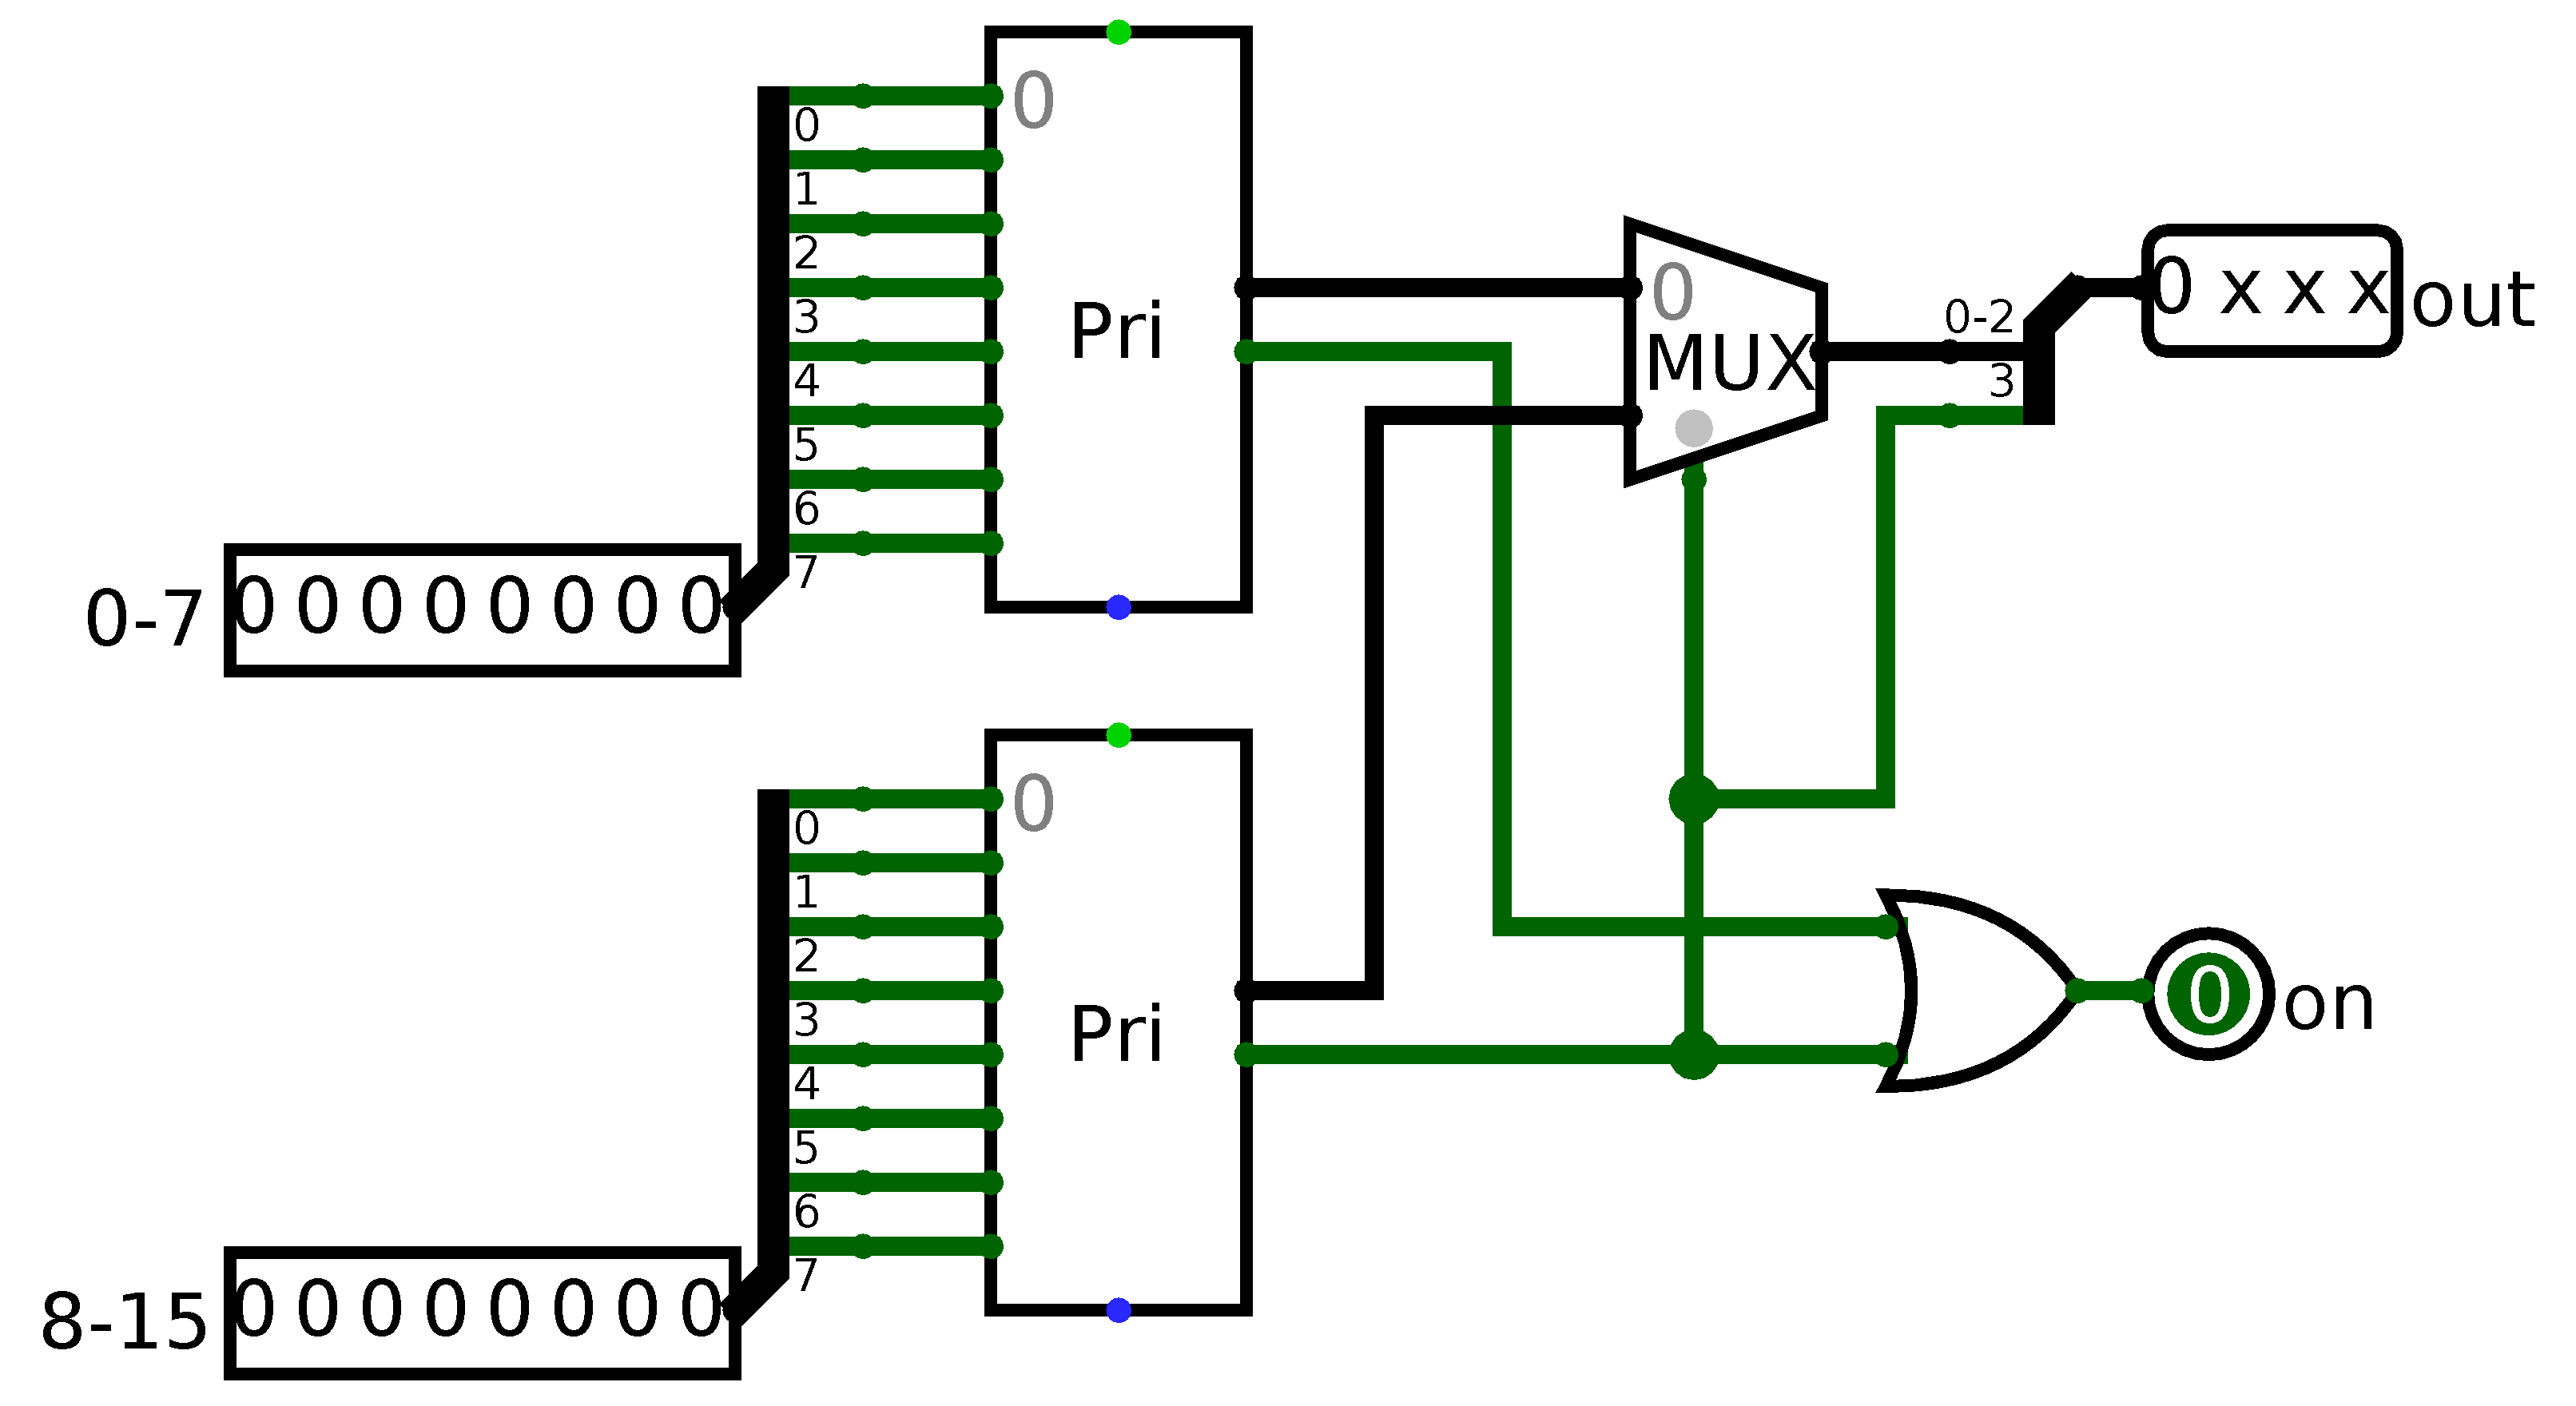
\includegraphics[width=0.5\textwidth]{assn/03/media/02.png}
      \caption{A 16-to-4 Encoder in Logisim}
    \end{figure}

    \item Implement a mod 6 counter using a ROM memory.
    \begin{figure}[h]
      \centering
      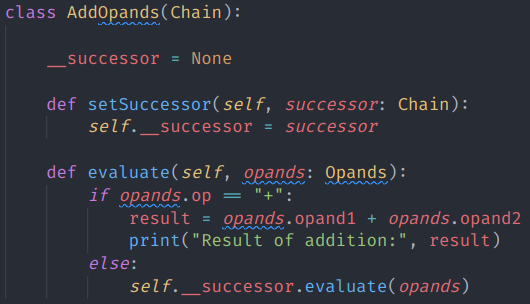
\includegraphics[width=0.5\textwidth]{assn/03/media/03.png}
      \caption{A Mod 6 Counter Using A ROM Memory in Logisim}
    \end{figure}

    \item Implement a stop light using a ROM memory.
    \begin{figure}[h]
      \centering
      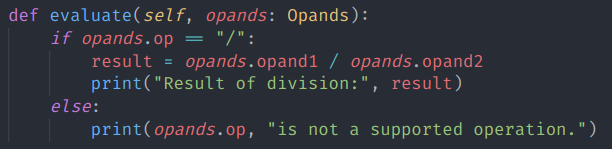
\includegraphics[width=0.5\textwidth]{assn/03/media/04.png}
      \caption{A Stop Light Using A ROM Memory in Logisim}
    \end{figure}

    \item Implement an 8-bit integer adder/subtracter using the circuit covered in class. 
    \begin{figure}[h]
      \centering
      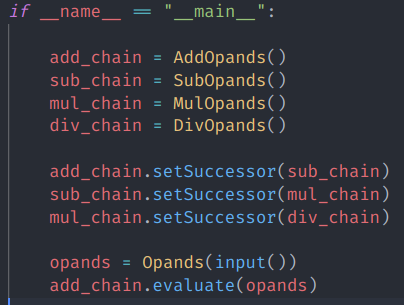
\includegraphics[width=0.4\textwidth]{assn/03/media/05.png}
      \caption{An 8-bit Integer Adder/Subtracter in Logisim}
    \end{figure}

  \end{enumerate}

\end{document}
